\documentclass[12pt]{article}
\usepackage{amsmath, amsthm, amsfonts, amssymb, bm}
\usepackage{graphicx,psfrag,epsf, float}
\usepackage{enumerate,titlesec, color}
\usepackage{natbib}
\usepackage{url} % not crucial - just used below for the URL 
\usepackage{soul}
\usepackage{subcaption}
\usepackage{booktabs}
\usepackage{tikz, geometry, tkz-graph, xcolor}
\usepackage{rotating}


\newcommand{\mX}{{\mathcal X}}
\newcommand{\mH}{{\mathcal H}}
\newcommand{\mZ}{{\mathcal Z}}
\newcommand{\tX}{{\widetilde X}}
\newcommand{\T}{{\mathcal T}}
\newcommand{\mS}{{\mathcal S}}
\newcommand{\mI}{{\mathcal I}}
\newcommand{\mU}{{\mathcal U}}
\newcommand{\hP}{{\widehat P}}
\newcommand{\hS}{{\widehat S}}
\newcommand{\sumi}{{\sum_{i=1}^n}}
\newcommand{\sumj}{{\sum_{j=1}^n}}
\newcommand{\sumk}{{\sum_{k=1}^n}}
\newcommand{\sumb}{{\sum_{b=1}^B}}
\newcommand{\mW}{{\mathcal W}}
\newcommand{\bX}{{\bm X}}
\newcommand{\bW}{{\bm W}}
\newcommand{\bV}{{\bm V}}
\newcommand{\bw}{{\bm w}}
\newcommand{\bA}{{\bm A}}
\newcommand{\bU}{{\bm U}}
\newcommand{\ba}{{\bm a}}
\newcommand{\bx}{{\bm x}}
\newcommand{\bz}{{\bm z}}
\newcommand{\bZ}{{\bm Z}}
\newcommand{\bM}{{\bm M}}
\newcommand{\CON}{{\rm CON}}
\newcommand{\TPR}{{\rm TPR}}
\newcommand{\FPR}{{\rm FPR}}
\newcommand{\NA}{{\rm NA}}
\newcommand{\ICON}{{\rm ICON}}
\newcommand{\wA}{{\widetilde A}}
\newcommand{\tL}{{t_{\rm L}}}
\newcommand{\bt}{{\bm t}}
\newcommand{\DeltaL}{{\Delta_{\rm L}}}
\newcommand{\bmkappa}{ {\bm \kappa} } 
\newcommand{\blue}[1]{\textcolor{blue}{#1}}
\newcommand{\red}[1]{\textcolor{red}{#1}}
\newcommand{\green}[1]{\textcolor{green}{#1}}
\newcommand{\cy}[1]{\textcolor{magenta}{#1}}
\newcommand{\vp}{\vspace{0.1in}}
\newcommand{\ns}{\normalsize}
\newcommand{\fn}{\footnotesize}
\newcommand{\scr}{\scriptsize}

\definecolor{firstposColor}{HTML}{FFb2b2}
\definecolor{chronicColor}{HTML}{FF3232}
\definecolor{mucoidColor}{HTML}{990000}
\definecolor{MDRColor}{HTML}{934c93}

\newcommand\crule[3][black]{\textcolor{#1}{\rule{#2}{#3}}}
\newcommand{\tikzcir}[2][black,fill=black]{\tikz[baseline=-0.5ex]\draw[#1,radius=#2] (0,0) circle;}
\newcommand{\lineCir}[2][]{\tikz[baseline=-.5ex]{\draw[#1, line width = 2pt](-.4,0) --(.4,0);\draw[#1, fill = #1] (0, 0) circle (#2);}}
\newcommand{\dashlineCir}[2][]{\tikz[baseline=-.5ex]{\draw[#1, dotted, line width = 2pt](-.4,0) --(.4,0);\draw[#1, fill = #1] (0, 0) circle (#2);}}
\newcommand{\openCir}[1][]{\tikz[baseline=-.5ex]{\draw[black,line width = 1pt] (0, 0) circle (#1);}}
\newcommand{\solidCir}[2][]{\tikz[baseline=-.5ex]{\draw[#1, fill = #1] (0, 0) circle (#2);}}
\newcommand{\solidDia}[2][]{\tikz[baseline=-.5ex]{\draw[#1, fill = #1] (#2,0) -- (0,#2) -- (-#2,0) -- (0,-#2) -- cycle;}}
\newcommand{\solidTri}[2][]{\tikz[baseline=-.5ex]{\draw[#1, fill = #1] (0,#2) -- (-0.86*#2, -0.5*#2) -- (0.86 * #2, -0.5*#2) -- cycle;}}

\newcommand{\mR}{{\mathcal R}}
\newcommand{\TL}{{T_{\rm L}}}
\newcommand{\YL}{{Y_{\rm L}}}
\newcommand{\YLi}{{Y_{{\rm L}i}}}
\DeclareMathOperator{\dev}{d\!}
\DeclareMathOperator{\E}{E\!}
\DeclareMathOperator{\logit}{logit\!}


\begin{document}

\begin{figure}
\centering
    \resizebox{.8\textwidth}{!}{
      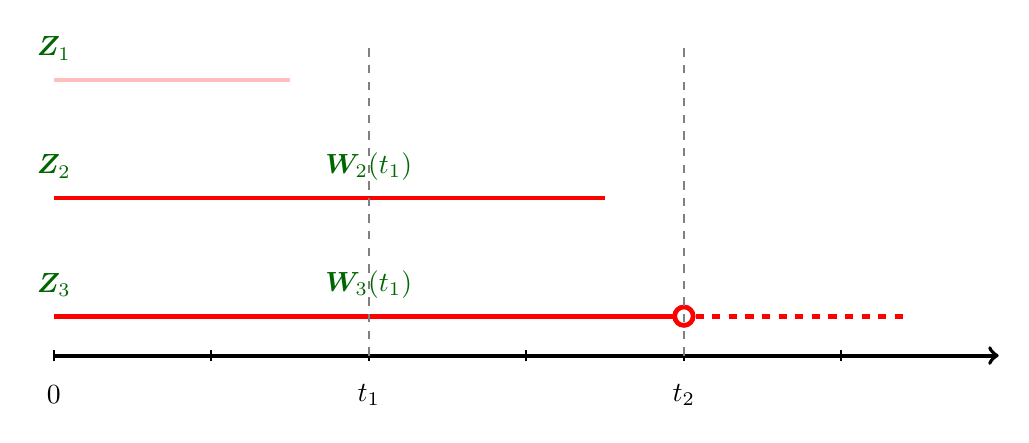
\begin{tikzpicture}
        \draw[line width = .5mm, ->] (0, -.5) -- (12, -.5);
        \draw[red, line width = .6mm, -o] (0, 0) -- (8.15, 0);
         \draw[red, line width = .6mm, dashed] (8.15, 0) -- (10.8, 0);
        \draw[red, line width = .6mm] (0, 1.5) -- (7, 1.5);
        \draw[pink, line width = .6mm] (0, 3) -- (3, 3);
        \foreach \y in {0,2,...,10}
        \draw[line width = .3mm] (\y, -0.075-.5) -- (\y, 0.075-.5);
        \node[black] at (0, -1) {0};
        \node[black] at (4, -1) {$t_1$};
        \node[black] at (8, -1) {$t_2$};
        \draw[dashed, gray, line width = .28mm] (4, -.5) -- (4, 3.5);
        \draw[dashed, gray, line width = .28mm] (8, -.5) -- (8, 3.5);
        %\draw[line width = 3.5mm, cyan!60!gray, opacity = 0.45] (2, -.5) -- (4, -.5);
        %\draw[line width = 3.5mm, black!60!green, opacity = 0.45] (0, -.5) -- (2, -.5);
        \node[black!60!green] at (0, .4) {\normalsize $\bZ_3$};
        \node[black!60!green] at (4, .4) {\normalsize $\bW_3(t_1)$};
        \node[black!60!green] at (0, 1.9) {\normalsize $\bZ_2$};
        \node[black!60!green] at (4, 1.9) {\normalsize $\bW_2(t_1)$};
        \node[black!60!green] at (0, 3.4) {\normalsize $\bZ_1$};
        \end{tikzpicture}}
\end{figure}


\end{document}

% o-
% *-

        \draw[line width = .75mm, blue!80!gray] (7, -.15) -- (7, .15);
        \node[blue!80!gray] at (7, -.4) {\normalsize $\boldsymbol{t_1 = 7}$};
        \draw[line width = .75mm, black!80] (4.84, -.15) -- (4.84, .15);

        \draw[line width = 3.5mm, cyan!60!gray, opacity = 0.45] (7, 0) -- (11.7, 0);
        \node[black!60!green] at (7.7, .4) {\normalsize $\boldsymbol{W(t_1) = 19.7}$ kg};
        \node[black!60!green] at (4.84, .4) {\normalsize $\boldsymbol{U_1 = 4.8}$};        
        
        